\section{The model}

This article deals with non-linear stochastic dynamical system in discrete-time.
The authors model with such systems with five sequences :
$x=(x_t)_{t=1\cdots T}$, $y=(y_t)_{t=1\cdots T}$, $u=(u_t)_{t=1 \cdots T}$, $w=(w_t)_{t=1 \cdots T}$ and $v=(v_t)_{t=1 \cdots T}$.

\begin{itemize}
  \item $u_t$ (in $\mathbb{R}^p$) are called the input variable and are observed.
  \item $x_t$ (in $\mathbb{R}^q$) are called the state and are unknown.
  \item $y_t$ (in $\mathbb{R}^n$) are called the output and are observed.
  \item $w_t$ and $v_t$ (in $\mathbb{R}^q \times \mathbb{R}^n$) are Gaussian noises and are unknown.
\end{itemize}

The stochastic dynamics equations are:
\begin{eqnarray}
x_{t+1}&=& f(x_t,u_t)+w_t\\
y_t &=& g(x_t,u_t)+v_t
\end{eqnarray}
and can be represented with the graphical model:
\begin{figure}[H]
	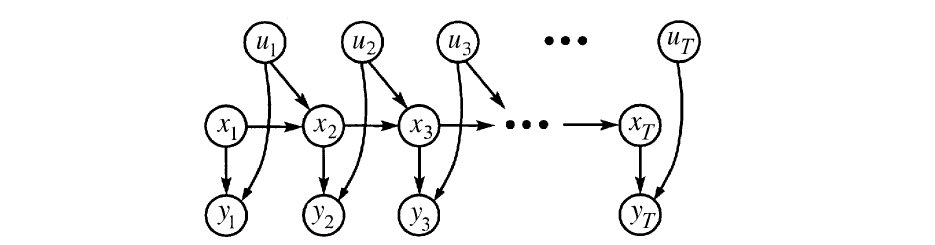
\includegraphics[width=14cm]{screenshot_graphical_model.PNG}
	\captionof{figure}{Graphical model of our system.}
\end{figure}
